\documentclass[10pt,a4paper]{article}

\usepackage[utf8]{inputenc}
\usepackage[T1]{fontenc}
\usepackage[french,english]{babel}
\usepackage{blindtext}

\usepackage[hyphens]{url}
\usepackage{hyperref}
\DeclareUrlCommand\email{\urlstyle{rm}}

\usepackage[margin=2in]{geometry} % showframe
\usepackage{multicol}

\usepackage{graphicx}
\usepackage{xcolor}
\usepackage{amsmath}
\usepackage{amsthm}
\usepackage{amsfonts}
\usepackage{amssymb}
\usepackage{siunitx}
\usepackage{pdflscape}
%\usepackage[toc]{glossaries} % https://www.overleaf.com/learn/latex/Glossaries
%\usepackage{parskip} % empty line between paragraphs
\usepackage{listings}
\usepackage{float}
\usepackage{pmboxdraw}
\usepackage{textcomp} % for the apostrophe
\usepackage{float}
\usepackage{comment}

% hyperref setup
\definecolor{darkgreen}{RGB}{0,180,0}
\hypersetup{
    colorlinks = true,
    linkbordercolor = {white},
    linkcolor = red,
    anchorcolor = black,
    citecolor = darkgreen,
    filecolor = cyan,
    menucolor = black,
    runcolor = cyan,
    urlcolor = magenta
}

% Bib setup
\usepackage{csquotes} % Recommended by biblatex
\usepackage[style=numeric,sorting=none,backend=biber]{biblatex}
\DeclareBibliographyAlias{software}{online}
\addbibresource{references.bib} % The file containing our references, in BibTeX format


\newcommand{\htriple}[3]{\ensuremath{\{#1\}~#2~\{#3\}}}
\newcommand{\WP}{\ensuremath{\mathit{WP}}}
\newcommand{\notimplies}{%
  \mathrel{{\ooalign{\hidewidth$\not\phantom{=}$\hidewidth\cr$\implies$}}}}
\newcommand{\eqdef}{\stackrel{def}{=}}

% \renewcommand{\implies}{\ensuremath{\Rightarrow}}

\newtheorem{theorem}{Theorem}[section]
\newtheorem{corollary}{Corollary}[theorem]
\newtheorem{lemma}[theorem]{Lemma}
\newtheorem{remark}{Remark}
\newtheorem*{remark*}{Remark}

%% Listing settings
\definecolor{codegreen}{rgb}{0,0.6,0}
\definecolor{codegray}{rgb}{0.5,0.5,0.5}
\definecolor{codepurple}{rgb}{0.58,0,0.82}
\definecolor{codeblue}{rgb}{0.10,0,0.82}
\definecolor{codebackcolour}{rgb}{0.95,0.95,0.92}
 


\title{Experiments on automation of formal verification of devices at the binary level}
\author{Thomas Lacroix --- \email{thomas.lacroix@insa-lyon.fr}\medskip\\
Département Informatique\\
INSA de Lyon}
\date{2018/2019}

\begin{document}

\newgeometry{margin=2cm}

\maketitle
\thispagestyle{empty}

{
\noindent Sous la responsabilité de :\\
\indent Mads Dam : Division of Theoretical Computer Science -- KTH\\
\indent Pierre-\'Edouard Portier : Département Informatique -- INSA Lyon
}

\vspace{\baselineskip}\vspace{\baselineskip}

{ % Block used for font size in abstracts
\fontsize{9}{10.8}

\begin{abstract}
  \rightmargin=1cm \leftmargin=1cm
  With the advent of virtualization, more and more work is put into the verification of hypervisors. Being low-level softwares, such verification should preferably be performed at binary level. Binary analysis platforms are being developed to help perform these proofs, but a lot of the work has to be carried out manually.

  In this thesis, we focus on the formal verification of a Network Interface Controller (NIC), more specifically we look at how to automate and reduce the boilerplate work from an existing proof. We base our work on the HolBA platform, its hardware-independent intermediate representation language BIR and supporting tools, and we experiment on how to perform this proof by leveraging existing tools.

  We first replaced the existing NIC model written in HOL4 to an equivalent one written using BIR, enabling the use of HolBA tools. Secondly, we developed some visualization tools to help navigate and gain some insight into the existing proof and its structure. Thirdly, we experimented with the use of Hoare triples in conjunction with an SMT solver to perform contract verification. Finally, we proved a simple contract written in terms of the formal NIC model on the BIR implementation of this model, unlocking the way of performing more complex proofs using the HolBA platform.
\end{abstract}

\leftmargin=1cm
{\small\textbf{\textit{Keywords---}} binary analysis, formal verification, proof producing analysis, theorem proving}

\vspace{\baselineskip}\vspace{\baselineskip}

\begin{otherlanguage}{french}
  \begin{abstract}
    \rightmargin=1cm \leftmargin=1cm
    Avec la démocratisation de la virtualisation, de plus en plus d'efforts sont consacrés à la vérification des hyperviseurs. S'agissant de logiciels de bas niveau, une telle vérification devrait de préférence être effectuée au niveau binaire. Des plates-formes d'analyse binaire sont en cours de développement pour aider à réaliser ces preuves, mais une grande partie du travail doit encore être effectuée manuellement.

    Dans cette thèse, nous nous concentrons sur la vérification formelle d'un Contrôleur d'Interface Réseau (NIC), plus spécifiquement sur la manière d'automatiser et de réduire le travail répétitif d'une preuve existante. Nous nous basons sur la plate-forme HolBA, son langage de représentation intermédiaire indépendant du matériel, BIR et ses outils de support, et nous nous intéressons à la manière de réaliser cette preuve en utilisant des outils existants.

    Nous avons d'abord remplacé le modèle NIC existant écrit en HOL4 par un modèle équivalent écrit en BIR, permettant ainsi l'utilisation des outils de HolBA. Deuxièmement, nous avons développé des outils de visualisation pour nous aider à naviguer et à mieux comprendre la preuve existante et sa structure. Troisièmement, nous avons expérimenté l'utilisation des triplets de Hoare en conjonction avec un solveur SMT pour effectuer une vérification par contrat. Enfin, nous avons prouvé un contrat simple écrit en termes du modèle formel du NIC sur l'implémentation de ce modèle en BIR, ouvrant la voie à la réalisation de preuves plus complexes avec la plate-forme HolBA.
  \end{abstract}
\end{otherlanguage}

\leftmargin=1cm
{\small\textbf{\textit{Mot-clés---}} binary analysis, formal verification, proof producing analysis, theorem proving}
}

\vspace{\baselineskip}\vspace{\baselineskip}

\restoregeometry
\newgeometry{margin=3cm}
\fontsize{10}{12}\selectfont
%--------------------------

\begin{multicols}{2}

\section{Introduction}
\textit{This section serves as an introduction to the degree project and presents the background of the work along with this thesis objective. Delimitations to the project and the choice of the methodology are also discussed.}

\subsection{Background}

Embedded systems are becoming more and more common with the current advent of {IoT} and mobile computing platforms, such as smartphones. Those systems are fully-fledged computers with powerful hardware, complete operating systems, and access to the Internet. Such systems can run security-critical services, such as a building security system or automatic toll gates, or carry valuable information as it is the case for personal smartphones. Therefore, these two characteristics make them targets of choice for attackers.

The {PROSPER} project \cite{noauthor_prosper:_nodate-1} aims to develop a secure and formally verified hypervisor for embedded systems. Hypervisors are thin layers running directly on top of hardware providing the ability to run virtualized applications, such that operating systems or real-time control systems. Those virtualized applications then don't have privileged access to the hardware and have to go through the hypervisor. This allows different applications to share the same hardware while providing strong isolation between them, thus ensuring confidentiality and security. Moreover, security not only means protection from external attacks but also resilience to bugs. If multiple critical systems are running on the same hardware, bugs or crashes in some systems shouldn't affect the others from behaving correctly.

Previous work in the {PROSPER} project achieved to formally verify a simple separation kernel \cite{dam_formal_2013}, which later resulted into an implementation of a working hypervisor. Then, they achieved to run both Linux and {FreeRTOS} on top of it. Finally, they formally verified memory isolation for virtualized applications \cite{nemati_trustworthy_2015}. However, hardware devices were not included in the verification, so devices, like Network Interface Controller ({NIC}), cannot be used by the virtualized applications reducing the value of the hypervisor. In order to solve this issue, verification of hardware devices is being carried out.

A formal model of a {NIC} device has already been produced, on which some security theorems have been proved \cite{haglund_formal_2016}. These theorems can be seen as high-level proofs relying on a layer of lower-level lemmas. This layer provides an abstraction over the raw formal model. This is illustrated in the left-hand side of Figure \ref{hol-v-bir-nic-model-simple}. However, there exist more devices that are of interest to verify, so it is very desirable to automate formal verification of devices and use a standard model for reasoning about them.

\begin{figure}[H]
  \centering
	\includegraphics[height=6cm]{figures/hol-v-bir-nic-model-simple.png}
	\caption{Formal v. BIR NIC models. The left hand side already exists. The dashed elements represent the work done during this project.}
	\label{hol-v-bir-nic-model-simple}
\end{figure}

The team is now developing a new framework for performing binary analysis in HOL4, an interactive theorem prover, named {HolBA} \cite{noauthor_holba_2019}. This framework features a machine-independent Binary Intermediate Representation (BIR), a proof-producing transpiler from ARMv8 and Cortex-M0 assembly code to BIR, called the lifter, a proof-producing weakest precondition generator for loop-free programs, and supporting tools \cite{metere_sound_2017,lindner_trabin:_2019}.

The idea of this work is to translate the formal {NIC} model of \cite{haglund_formal_2016} using {BIR}, then use HolBA's proof-producing weakest precondition tool to prove the same lower-level lemmas than the formal model. With all the lemmas proved, the security properties are implied. Figure \ref{hol-v-bir-nic-model-simple} gives an overview of this idea: using the proof-producing weakest precondition tool to bind together a newly written BIR NIC model and the work done on the formal model.

\subsection{Thesis objective}

The goal of this thesis project is to explore verification techniques in order to automate parts, if not all, of the verification process of hardware devices using the HolBA platform. The formal {NIC} model of \cite{haglund_formal_2016} is used as working example.

\subsection{Delimitations}

This work being about exploration of techniques towards automation of verification techniques, instead of being about producing an actual complete proof of a hardware device, some implementations have not been completed in order to save time to explore in more areas. Additionally, this work mainly concerns the HolBA platform that is developed in the team where this thesis took place.

\subsection{Choice of methodology}

This work has been carried out step-by-step toward an ideal goal, i.e. re-establishing all the security properties. On the road, needs have been identified and tools have been implemented in order to tackle them. This approach made sense in this particular work because the needs were not known in advance, and therefore needed to be identified. This thesis presents the steps taken during this work, the motivations of each tool that have been implemented, and discusses their limitations and future work in the conclusion.

\subsection{Related work}

\subsubsection{Secure execution platforms}

The {PROSPER} project isn't the only project focused on high-security execution platforms. Platforms such that seL4, Microsoft Hyper-V, INTEGRITY Multivisor or even MINIX 3 are examples of platforms used in production and providing strong security properties.

\paragraph{seL4} is a recent L4-based microkernel created in 2006 with the goal to produce a completely formally verified implementation of an L4 microkernel. This has been achieved in 2009 \cite{klein_sel4:_2009}. At this time, seL4 consisted of \num{8700} lines of C code and \num{600} lines of assembler. The implementation of seL4 has been formally proved from its abstract specification down to its C implementation. Later, the validity of the generated assembly code has been proved, removing the need of trusting the compiler \cite{noauthor_what_nodate}.

\paragraph{Microsoft Hyper-V} is Microsoft's hypervisor, widely used today within the Microsoft Azure cloud platform. It has been released in 2008. Hyper-V is a huge codebase, as we can read on VCC's website \footnote{\url{https://www.microsoft.com/en-us/research/project/vcc-a-verifier-for-concurrent-c/}}: ``Hyper-V consists of about 60 thousand lines of operating system-level C and x64 assembly code, it is therefore not a trivial target''. Microsoft has put a lot of work in formal verification\footnotemark of Hyper-V down to machine code \cite{leinenbach_verifying_2009}. However, they don't appear to include device drivers in their formal verification.

\footnotetext{Microsoft has several formal verification projects, many of which are freely available for non-commercial use: \url{https://github.com/Microsoft?q=verifier}}

\paragraph{INTEGRITY Multivisor} is a commercial real-time operating system and hypervisor developed by Green Hills Software. Although not much information seems to be publicly available, Green Hills Software has done considerable formal verification work \cite{richards_modeling_2010}. Multivisor has several certifications, including, for example, ISO 26262 ASIL D automotive electronics, NSA-certified secure mobile phones or FAA DO-178B Level A-certified avionics controlling life-critical functions on passenger and military aircraft \footnote{\url{https://ghs.com/products/rtos/integrity_virtualization.html}}.

\paragraph{MINIX 3} is an operating system whose design is focused on high reliability and security. It is based on a tiny microkernel with the least responsibility possible, and the rest of the operating system is running an a number of isolated user processes. MINIX 3 has not been formally verified, but intends to provide strong security guarantees by design.

\subsubsection{Binary analysis platforms}

For this project, we will use the {HolBA} framework. However, several other binary analysis platforms have been created for various purposes, such as formal verification or static analysis. A common characteristic of these platforms is their use of an Intermediate Representation ({IR}). IRs are designed to be simpler to use for each platforms' end purpose. As an example, the HolBA platform has BIR as its intermediate representation.

\paragraph{Microsoft Boogie} is Microsoft's intermediate verification language. Boogie is the IR for multiple Microsoft tools, including VCC. Boogie as a tool can infer some invariants on the given Boogie program and then generate verification conditions that are passed to an SMT solver \footnote{\url{https://www.microsoft.com/en-us/research/project/boogie-an-intermediate-verification-language/}}.

\paragraph{Valgrind} is a framework for building program supervision tools, such as memory checkers, cache profilers or data-race detectors \cite{nethercote_valgrind:_2003}. As its core, Valgrind is a JIT x86-to-x86 compiler, translating binary programs into its IR called UCode. Then, \textit{skins}---tools built using the Valgrind framework---are free to work with the IR in order to perform their analysis.

\paragraph{LLVM} is a compiler infrastructure which supports a unique multi-stage optimization system \cite{lattner_llvm:_2002}. LLVM is built around its {IR}, LLVM Virtual Instruction Set, which can be described as a strict RISC architecture with high-level type information. This IR made LLVM successful because it is a pragmatic IR suitable for optimizations at multiple stages (link-, post-link, and run-time) and supporting a wide variety of transformations. Leveraging this IR, an ecosystem grew around LLVM, providing tools such as symbolic execution (LLVM KLEE), benchmarking environments or static and dynamic analyzers.

\paragraph{Mayhem} is a system for automatically finding exploitable bugs in binary programs and generating working exploits as proof of the discovered vulnerabilities \cite{cha_unleashing_2012}. It leverages BAP, the Binary Analysis Platform from Carnegie Mellon University (CMU BAP) \cite{brumley_bap:_2011}, as its IR. It proceeds by fist JIT-ing each instruction to the BAP intermediate language (IL) and then performing a custom symbolic execution.
\medskip

There are several other tools, platforms, and frameworks, such as Angr. An interesting note though is that BIR's design is based upon CMU BAP's intermediate language.

The novelty introduced in HolBA, however, is that proofs are performed directly on the generated assembly code, not at the source code level. Therefore, proofs can be performed on programs without needing their source code, and regardless on the programming language used as long as it can be compiled in assembly code in an {ISA} supported by the platform.

\section{Definitions and relevant theories}
\textit{This section intends to provide brief introductions for concepts and the foundation of theories that are essential in order to understand the problem that this project aims to explore.}

\subsection{Interactive Theorem Proving and HOL4} \label{hol4-presentation}

Interactive theorem provers are software producing formal proofs, in an
interactive fashion, i.e. a human can step through the proof interactively while the proof assistant provides some automation (like rewriting of terms, arithmetic evaluation, or integration with external tools like SMT solvers). Coq, HOL4 or Isabelle are such tools.

HOL4 \cite{noauthor_hol_nodate} stands for Higher-Order Logic. It is a programming environment deeply embedded into the {SML} programming language enabling to prove theorems and write {proof-producing} programs. HOL4 uses a very small kernel in order to provide very high guarantees of correctness.


\subsection{HolBA's BIR} \label{bir-presentation}

HolBA's Binary Intermediate Representation (BIR) \cite{lindner_trabin:_2019}, introduced in the Introduction, is a machine independent binary representation. It aims to be the simplest possible while still being able to represent all possible binary programs but self-modifying programs. It does so by having a limited syntax and by forbidding implicit side-effects. A statement can only have explicit state changes and can only affect one variable. Valid BIR programs must be well-typed.

This representation allows producing proofs more easily that with classical binary representations, whose design are focused on execution speed rather than offline analysis. Moreover, BIR doesn't have unspecified behavior.

BIR is implemented as a set of HOL4 data types, and possesses a completely defined semantic. Section \ref{bir-memories-with-smt-solvers} contains a more thorough discussion of the BIR semantic. Section \ref{alice-bob-toy} implements a toy BIR program and presents the concrete BIR syntax.

Among its supporting tools, HolBA features a tool to visualize the Control Flow Graph ({CFG}) of BIR programs.

\subsection{Hoare Triples} \label{hoare-triples}

For a given program $prog$ consisting of a list of instructions and two predicates $P$ and $Q$ called respectively pre- and postcondition, a Hoare Triple \htriple{P}{prog}{Q} states that when executing the program $prog$ from a state $S$ terminates in a state $S'$, if $P$ holds in $S$ then $Q$ will hold in $S'$ (Equation \ref{ht_def}). Hereafter, we assume programs and states to be well-typed. A Hoare Triple is also called \textit{a contract}.
\begin{multline}
  \htriple{P}{prog}{Q} \eqdef\\
  S' = exec(S, prog) \land P(S) \implies Q(S')
  \label{ht_def}
\end{multline}

For example, \htriple{P}{\varnothing}{P} holds because an empty program doesn't change the state of the execution. \htriple{n=1}{n:=n+1}{even(n)}, with $n \in \mathbb{N}$, holds because $1+1=2$, which is even.

\subsection{Weakest preconditions}

While Hoare logic introduces sufficient preconditions, Dijkstra introduced the concept of necessary and sufficient preconditions, called ``weakest'' preconditions \cite{dijkstra_guarded_1975}. Such weakest preconditions (WP) can be automatically derived from a program $prog$ and a postcondition $Q$. Let's call $\WP(prog, Q)$ such a WP. Then, from Equation \ref{ht_def} follows:
\begin{equation}
  \forall (prog, Q),
  \htriple{\WP(prog,Q)}{prog}{Q}
  \label{ht_wp_eq}
\end{equation}

For the program $n:=n+1$ mentioned in the previous section, the WP for the postcondition $even(n)$ is $odd(n)$, i.e. incrementing the value of an odd integer variable by one makes it even.

For a triple \htriple{P}{prog}{Q} to hold, $P$ must be stronger than the WP, i.e. we need to prove that $P \implies \WP(prog, Q)$. While multiple methods exist to perform such proofs, Satisfiability Modulo Theory ({SMT}) solvers offer a convenient and automatic solution. With an SMT solver, proving $R$ consist in checking that $\neg R$, its negation, is \textit{unsatisfiable}. SMT solvers can also give counter-example $R$ is false.

{HolBA} provides a {proof-producing} tool for automatically deriving WP on loop-free {BIR} programs whose control flow can be statically identified \cite{lindner_trabin:_2019}. However, SMT solvers had never been used before this work.


\section{Overview of the formal proof of the NIC model} \label{overview-nic-proof}
\textit{This section will present the formal verification of \cite{haglund_formal_2016} and present an attempt that have been made about visualization of the proofs.}
\medskip

The formal verification of a NIC in \cite{haglund_formal_2016} represents the NIC as a transition system. composed of five finite state automata, each responsible for a different task: initialization, transmission, transmission teardown, reception and reception teardown. These automata have autonomous transitions that represent the standalone operation of the device. Communication with the CPU is represented with non-autonomous transitions. The model also contains a scheduler. Since this model has been realized using the public specification of the device, which is underspecified, the simulated state of the device is marked \textit{dead} if the model is asked to describe any transition or operation that is not described by the specification.
Being designed as a transition system, the whole model is loop free, which is convenient for contract-based verification, since that hard composition theorems would otherwise be needed.

% TODO: Check that loop-free is mentioned afterwards

The state of the NIC is defined as a nested data type containing registers and a memory called \textit{CPPI\_RAM}.

The low-level lemmas of the verification (cf. Figure \ref{hol-v-bir-nic-model-simple}) are stated as Hoare Triples using invariants (Equation \ref{nic-proof-invariant-shape}) that must hold for every possible transition:
\begin{small}
  \begin{equation}
    \label{nic-proof-invariant-shape}
    I_{NIC} \eqdef \neg dead~\land~I_{init}~\land~I_{tx}~\land~I_{rx}~\land~\cdots
  \end{equation}
\end{small}

\subsection{Visualizing proof dependencies}

The model of the NIC consists of \num{1500} lines of HOL4 code and required around three man-months of work. The NIC invariant consists of \num{650} lines of HOL4 code and the proof consists of approximately \num{55000} lines of HOL4 code including comments. Identifying the invariant and implementing the proof in HOL4 required around one man-year of work \cite{haglund_trustworthy_nodate}.

The proof being consequent and divided into several script files, it is difficult to identify what are the low-level lemmas to be reproved in this work. Therefore, a tool, called DepGraph, has been implemented in order to extract the dependency structure from proof files in the form of a graph. Then, the fringe of the graph represents the smallest set of lemmas that is enough to prove in order to imply the security properties by using the rest of the proofs unchanged.

DepGraph features two frontends that can extract dependencies between HOL4 theories (i.e. compiled {SML} files containing proofs of lemmas and theorems) and between definitions, theorems, and lemmas. However, this tool presents some critical shortcomings:

\begin{itemize}
	\item The theory dependencies exporter uses files generated by Holmake, the HOL4 compile system, in order to get the dependencies between theories. However, those files don't really represent dependencies but the files to be loaded before this script can be loaded, in a recursive fashion. Therefore, they represent the transitive reduction of the dependency graph. Because of this fact, precious knowledge is lost and cannot be recovered by using this method: edges representing direct dependencies can be removed if the remaining edges still account for this dependency. Therefore, we are still able to tell which nodes depend on some node $n$, but we cannot identify the aforementioned fringe. In order to solve this problem, different approaches exist, such as implementing a simplified SML parser that looks only at dependencies, or injecting code inside the dependency resolution of an existing SML compiler. However, this would involve too much work that isn't the direct focus of this thesis.
	\item The definition, theorem and lemma dependencies exporter uses word-based heuristics in order to extract dependencies, and is as such not quite reliable and cannot give any guarantee. As above, there exist similar solutions in order to get multiple levels of guarantees, such that implementing a SML parser or injecting code inside HOL4 theory and definitions handling, but this would also require too much work. Destructuring HOL4 theories does not work because of how HOL4 has been designed. Moreover, such dependency graphs become quickly big, making them unusable in practice, and some additional work would be needed in order to represent them in a convenient way. Therefore, as above, no further work has been put into this exporter.
\end{itemize}

\noindent DepGraph's frontend for theory dependencies is still useful for documentation purpose, and has been used to visualize HolBA's architecture.

\section{The BIR NIC model} \label{nic-model}
\textit{This section presents the three different approaches made in order to implement an equivalent BIR model from the formal NIC model. Tools that have been implemented in order to build it will also be introduced.}
\medskip

Multiple approaches to the translation of the formal NIC model to an equivalent BIR program have been considered, from handwritting a BIR program (Sections \ref{alice-bob-toy} to \ref{impl-real-model}), lifting a C program (Section \ref{c-model}) to developing a new device model specific IR (Section \ref{flowchart-attempt}).

\subsection{Using flowcharts as Intermediate Representation} \label{flowchart-attempt}

The CFG of the transition system of the formal model looks like a tree. Therefore, using flowcharts could be a convenient way to represent such structures. An attempt has been made to design a flowchart representation. Figures \ref{flowchart-scheduler}, \ref{flowchart-tx} and \ref{flowchart-tx_fetch_next_bd} show respectively a preview of the scheduler, transmission automaton and a particular transition of this automaton.

However, while this visual representation is useful in order to get to know the formal NIC model, we encountered several shortcomings:

\begin{itemize}
    \item Flowcharts of each transition rapidly grows in size with the complexity of its formal counterpart. Possible workarounds include the use of nested diagrams, as it is the case of Figure \ref{flowchart-tx_fetch_next_bd} representing one node of Figure \ref{flowchart-tx}, namely \texttt{fetch\_next\_bd}, or usage of shorter ways of representing common patterns, as it is the case for representing dead transitions on Figure \ref{flowchart-tx_fetch_next_bd}.
    \item It is hard to define a coherent visual language able to represent the full set of features needed in order to realize device models. Additionally, this language must be compatible or easily translatable to BIR.
    \item It is hard to design a textual representation of this visual language other than conventional programming languages, so using such representation would require a substantial implementation effort in order to implement all the tools needed to use it. Developing visualization tools for a conventional language appears to be a more reasonable approach than developing a visual language.
\end{itemize}

For those reasons, it has been decided to not go further with this visual representation, and to focus instead of existing tools of the HolBA platform.

\subsection{Writing the model in C} \label{c-model}

One-to-one translation of the definitions related to the transmission automaton, scheduler, state, and \textit{CPPI\_RAM} of the formal model have been realized in C. However, when studying the compiled assembly code and lifted BIR program, we noticed that all the convenient naming that we can use in the formal or the C model is lost and replaced with abundant usage of the stack. While this is completely normal behaviour for a C compiler, this is not convenient when performing later proofs on the model. Reasoning about the stack would require more code than a complete rewrite of the model in BIR. This experiment made us realize that writing the model is a rapid operation and that we should rather focus on making the verification step as smooth as possible because it is the most difficult one to perform.

\subsection{A toy BIR model} \label{alice-bob-toy}

Before writing the whole NIC model by hand, we shall identify the structure of the model and develop tools that facilitate its implementation. Using well-designed tools can reduce the boilerplate work of the implementation, helping to focus only on the meaningful content of the implementation, and can also reduce the chance of introducing bugs as the code is factored and mechanically shorter.

A transition system similar to the one of the NIC model has been implemented, containing one scheduler and two automata. The two automata feature a simple linear transition system, and each of them has one non-autonomous transition, that is performed respectively by two external functions that represent memory accesses from the CPU in the NIC model.

This toy model has first been designed using the flowchart representation. Then, writing the BIR program has been a repetitive but straightforward step. The resulting BIR program is \num{450} lines of code long. The following issues have been identified:

\begin{itemize}
    \item BIR, as a HOL4 embedded language, is very verbose. Simple operations like additions or assignments require long constructions. Section \ref{bsl} presents BSL, a less verbose way of writing BIR programs.
    \item BIR features only one conditional statement controlling the control flow of a program: conditional jumps. Hence, BIR is not convenient for representing \textbf{if-then-else} statements with more than two branches. Section \ref{impl-real-model} presents some helper functions that have been implemented in order to be able to abstract the raw BIR code and work at a higher level.
\end{itemize}

\subsection{BSL: BIR Simple Language} \label{bsl}

A library, named BSL, offering the same expressiveness than BIR but with shorter constructs, has been implemented. This library has been kept simple and will serve as the base layer of possible later abstractions. As such, it has been decided that no feature other than pure syntactic construct, such that type inference, would be included.

BSL is composed of a set of functions with short names (prefixed with the letter \textit{b} in order to not clash with names in the global namespace) and a coherent interface offering interoperability with HOL4 quotation system and smart use of partial function application (e.g. for BIR types).

\subsection{Implementing the real model} \label{impl-real-model}

From the knowledge gained in \ref{alice-bob-toy}, a set of helper functions has been implemented, mainly in order to facilitate reasoning about the state machine.

Because of time constraints, not every transition of the formal NIC model have been implemented in this new model. Instead, we decided to focus on only some transitions in two automata: initialization and transmission. This focus is pragmatic for two reasons: (a) we decided to write the model along with the proof, only needed transitions for the current proof, in order to grow the model at a reasonable pace and to no clutter it with unneeded features or at the contrary missing critical aspects during the first sketch (b) as the verification was performed at the same time, we decided to start with easier, but not obvious, transitions, hence the choice to postpone verification of the more complex reception automaton to later in the work.

















































\section{Non-proof-producing automatic contract verification} \label{impl-non-pp-wp-lib}
\textit{This section presents the library that has been implemented in this work for automatic contract verification, after discussing about the problems that have been solved in order to build it.}

\subsection{Exporting BIR expressions to SMT solvers} \label{exporting-bir-to-smt}

% TODO TODO TODO TODO TODO TODO
% TODO: Is it said somewhere that the HT implications are BIR expressions?

In order to prove the implication needed to prove Hoare Triples, we must be able to export HOL4 goals to external SMT solvers. HOL4 features a library for interfacing {SMT} solvers and HOL4, called \textit{HolSmtLib}, using the standard format SMT-LIB 2.0 \cite{barrett_satisfiability_2016}. However, for obvious reasons, \textit{HolSmtLib} cannot export BIR expressions out of the box. Therefore, the BIR expression must be first translated.

As an intermediate language for formal verification, {BIR} possesses a precise semantic. The semantic of BIR expressions is expressed as a set of definitions describing what are the equivalent operations using HOL4's \textit{wordsTheory} and \textit{combinTheory}.

Because of the complexity of the BIR semantic, we deciced to implement a non proof-producing translation, in order to get more time for other experiments. The obvious downside of such a function is that we now have to trust the translation to be sound because we no longer get any guarantee from the theorem prover, but a proof-producing version can still be implemented later.

\textit{bir\_exp\_to\_words} has been implemented as an exhaustive \textit{match} statements on the expression type, each type being then translated to the corresponding non-BIR expression. Reccursive call is used for nested expressions.

\subsection{BIR memories and SMT} \label{bir-memories-with-smt-solvers}

% TODO: Swap this subsection with the previous one?

In order to prove Hoare Triples containing BIR memories, we need to use \textit{combinTheory}. However, it is not supported by \textit{HolSmtLib}. In order to solve this issue, we proceeded in two steps:

\begin{enumerate}
  \item we looked at how to translate BIR memory operations to SMT-LIB 2.0 and found \textit{ArraysEx}. Then, we verified that this translation is sound by checking that \textit{ArraysEx}'s axioms are correct in HOL4.
  \item we extended \textit{HolSmtLib} in order to support this theory, and wrote tests in order to ensure that the implementation is correct, since this library is not proof-producing \footnote{\textit{HolSmtLib} does have proof-reconstruction capabilities, but they are using an outdated version of Z3, the SMT solver that we used.}.
\end{enumerate}

\subsection{Pretty-printing of BIR expressions} \label{pretty-printers}

Generated WP grow in size quickly with the number of statements in a program, linearly or exponentially depending on the type of statements \footnote{Control flow statements produce exponential growth. While clever techniques can be implemented to keep their size reasonable \cite{lindner_trabin:_2019}, we often need to read and analyze them.}. Additionally, the default printing of BIR terms is very verbose. In order to increase user-friendliness, the readibility of long BIR expressions should be improved. Therefore, four pretty-printers have been implemented, providing the following features:

\begin{itemize}
    \item Simplification of verbose constructs.
    \item Different representation of \textbf{if-then-else} statements, simplifying reading the expression when either the condition or the \textbf{then} expression are very long.
    \item Consistent breaking of long expressions.
    \item Highlighting of types, facilitating debugging when the expression isn't well-typed.
    \item Highlighting of all strings, facilitating reading labels and variable names.
    \item Gathering of nested binary expressions of the same type at the same level.
    \item Rainbow parenthesis, i.e. matching pairs of parenthesis are printed in the same color. This feature is really useful when reading long expressions in order to quickly identify where a sub-expression ends.
\end{itemize}

\subsection{Implementing a convenient interface} \label{impl_convenient_ht_interface}

In order to perform a high number of proofs on the {NIC} model, we want to hide as much as possible the implementation details of the contract verification procedure. Ideally, we want a function ``\texttt{prove\_contract}'' taking a program fragment, a pre- and a postcondition as parameters, and producing a proof about the Hoare triple if the contract holds or a comprehensive and useful error message if it doesn't.

\begin{lstlisting}[
    language=Caml,
    backgroundcolor=\color{codebackcolour},
    keywordstyle=\color{magenta},
    label=interface_prove_contract,caption=Interface of ``\texttt{prove\_contract}'',
    frame=tb,basicstyle=\footnotesize\ttfamily]
fun prove_contract contract_name prog_def
    (precond_lbl, precond_bir_exp)
    (postcond_lbl_list, postcond_bir_exp)
\end{lstlisting}

When implementing this function, high attention has been paid to provide useful and comprehensive feedback in the case of failure. To that end, extensive use of exception wrapping has been made in order to give precise context to exceptions, and a logging library has been implemented (cf. Section \ref{user-friendliness}).

Then, in order to test this function and check that the interface actually let us verify different contracts, we verified three different programs:

\begin{enumerate}
  \item we verified \htriple{\top}{prog}{y = 100} on a simple program containing one conditional jump where each target assigns a different value to $y$, but where the condition is always true at runtime.
  \item on a program storing a number $N$ in memory at address $A$, then loading into $x$ from address $B$, we verified \htriple{A=B}{prog}{x=N}. This test allowed us to check that the extension of \textit{HolSmtLib} works for basic cases.
  \item on a program computing the sum of integers from $0$ to a given $n$ using a for loop, we verified the loop invariant on the body of the loop, using Gauss' formula.
\end{enumerate}

For each of those tests, we also experimented with other pre- and postconditions, and checked that invalid contracts can indeed not be proved.

\subsection{Simple automatized proofs on the NIC model} \label{simple-automated-proofs-on-nic}

Since the base lemmas of the formal NIC proof are phrased in terms of invariants holding in each transition of the model, representable as Hoare Triple, they can be proved using the non-proof-producing contract verification library that has been implemented in this project, as long as the pre- and postconditions can be represented using BIR.

We used \texttt{prove\_contract} in order to successfully verify two Hoare Triples (Equations \ref{nonpp-goal-1} and \ref{nonpp-goal-2}). Those two Hoare Triple respectively represent that, stating from a non-dead initial NIC state, performing one autonomous transition of the transmission automaton doesn't end in an undefined state (i.e. a dead state) and performing one non-autonomous transition of the initialization automaton does end in an undefined state.
\begin{multline}
  \{\neg NIC.dead~\land\\
  NIC.tx.state \in \{tx2,tx3,tx5,tx6,tx7\}\}\\
	tx\_automaton\{\neg NIC.dead\}
    \label{nonpp-goal-1}
\end{multline}
\begin{multline}
	\{\neg NIC.dead \land NIC.init.state \in \{it1,it3,it4\}\}\\
	init\_automaton\{NIC.dead\}
    \label{nonpp-goal-2}
\end{multline}

\subsection{Limitations of this approach}

While being convenient and working well for simple contracts, the contract verification library implemented in this chapter suffers from two limitations:

\begin{itemize}
  \item this library isn't {proof-producing}. Using HOL4 requires a significant learning effort, and easier non proof-producing tools exist.
	\item this library, with its approach to contract-based verification, is limited by the expressiveness of BIR, since the pre- and postconditions are BIR terms. BIR doesn't have quantifiers, and it is, therefore, impossible to prove contracts containing existential quantifiers. The existing formal proof on the NIC of \cite{haglund_formal_2016} requires existential quantifiers in order to reason about the buffer descriptor queue in the \textit{CPPI\_RAM} memory of the NIC, and this part of the proof can therefore not be replaced by using \texttt{prove\_contract}.
\end{itemize}

The following Section \ref{trustful-nic-analysis} explores a new proof-producing approach for performing contract-based verification on the BIR model that gives an answer to these issues.







































\section{A new approach for trustful analysis} \label{trustful-nic-analysis}
\textit{In this section, we will perform a proof on a BIR program and then lift it to an abstract model.}
\medskip

In order to prove the feasibility of the approach, we decided to prove a simple property. We used as a formal state, on which we want to prove a property, a HOL4 data type composed of two variables: $NIC.dead:bool$ and $NIC.x:word32$. Equations \ref{proof_nic_P_def}, \ref{proof_nic_Q_def} and \ref{proof_goal} present the property that we proved. Listing \ref{proof_prog} contains a pseudocode representation of the BIR program on which we performed the verification. Figure \ref{proof_schema} represents visually the structure of the verification and the steps that we took during the proof.
%
\begin{small}
\begin{align}
  \begin{split}
    \label{proof_nic_P_def}
    \vdash~\forall &nic.~P_{NIC}~nic \eqdef\\
      &~~~~~\neg nic.dead \land nic.x = 0w
  \end{split}\\
  %
  \begin{split}
    \label{proof_nic_Q_def}
    \vdash~&\forall nic~nic'.~Q_{NIC}~nic~nic' \eqdef\\
      &~~~~~\neg nic'.dead \land nic'.x = nic.x + 1w
  \end{split}\\
  %
  \begin{split}
    \label{proof_goal}
    \vdash~&\forall nic~nic'.~(exec\_prog~nic~bir\_prog~nic'\\
      &\land~P_{NIC}~nic)~\implies~Q_{NIC}~nic~nic'
  \end{split}
\end{align}
\end{small}
%
\begin{lstlisting}[
    language=C,
    backgroundcolor=\color{codebackcolour},
    commentstyle=\color{codegreen},
    keywordstyle=\color{magenta},
    stringstyle=\color{codepurple},
    label=proof_prog,caption=Pseudocode of the program used in this proof,
    frame=tb,basicstyle=\footnotesize\ttfamily]
nic.x := nic.x + 1
if nic.x > 10:
    nic.dead := true
\end{lstlisting}
%
\begin{figure}[H]
	\includegraphics[width=\columnwidth]{figures/proof_schema.png}
	\centering
	\caption{Visual structure of the proof. References like (a) to the arrows of this Figure are used throughout the proof to refer to a particular step.}
	\label{proof_schema}
\end{figure}
%
\begin{remark} \label{remark_Q_nic_intial_final}
$Q_{NIC}~nic~nic'$ has been defined on both initial and final states, in order to be able to reason about the initial state in the postcondition. This allowed us to write $nic'.x = nic.x + 1w$ instead of $nic'.x = 1w$ for example.
\end{remark}
%
\par We used Definition \ref{proof_eq_thm} in order to establish a relation between the HOL4 definition (a) and the BIR program (c). Another solution would have been to generate a proof-producing lifter from the formal definition (a) to BIR program (c), but has been kept as future work.
%
\begin{small}
  \begin{equation}
  \begin{split}
    \vdash \forall &nic~nic'.~exec\_prog~nic~bir\_prog~nic'~\eqdef ~~\, \mathbf{(a)}\\
      &\forall bir\_state~bir\_state'.~(R~nic~bir\_state~\land ~~ \mathbf{(b)}\\
            &~~~~bir\_state' = BIR\_exec~prog~bir\_state) ~~ \mathbf{(c)}\\
            &~\implies R~nic'~bir\_state' ~~~~~~~~~~~~~~~~~~~~~~~~~~~\, \mathbf{(d)}
  \end{split}
  \label{proof_eq_thm}
  \end{equation}
\end{small}
%
\vspace{-5pt}
\par The relation $R$ is used to express an equivalence between HOL4 states (``$nic$'') and BIR states, and is defined as a simple mapping of the variables between the BIR state and the formal state.

\begin{proof}

For (b), we proved the injectivity of $R$, and added to the theorem some constraints on the initial BIR state needed as hypothesis for $BIR\_exec$.

Then, we defined the equivalent pre- and postcondition on BIR, and proved Theorem \ref{proof_b_thm}.
%
\begin{equation} \label{proof_b_thm}
  \begin{split}
  \vdash~\forall bir\_state~(\exists nic.~R~nic~bir\_state~\land\\
  P_{NIC}~nic) \implies P_{BIR}~bir\_state
  \end{split}
\end{equation}
  
\paragraph{Limitation} $Q_{BIR}$ is a function of the end state only. Hence, in order to reason about the initial state, we need in general to introduce ghost variables postcondition. In this proof, since the contract that we are proving is simple, using the actual value of $nic.x$ is enough. However, this may pose a problem if we want to generalize the proof.

For step (d), we proved Theorem \ref{proof_d_thm}. We introduced $bir\_state$ and $P_{BIR}$ in order to reason about both the initial and final state in the postcondition (cf. Remark \ref{remark_Q_nic_intial_final}).
%
\begin{equation} \label{proof_d_thm}
\begin{split}
\vdash~\forall~&bir\_state'.~Q_{BIR}~bir\_state' \implies\\
	&(\forall nic~nic'~bir\_state.~P_{BIR}~bir\_state\\
	&~~~~~~\land~R~nic~bir\_state~\land~R~nic'~bir\_state'\\
	&~~~\implies Q_{NIC}~nic~nic')
\end{split}
\end{equation}

Finally, we proved that the Hoare Triple holds on the BIR program:

\begin{equation} \label{proof_ht_thm}
\vdash~\htriple{P^{exp}_{BIR}}{bir\_prog}{Q^{exp}_{BIR}}
\end{equation}

To that end, we used HolBA's proof-producing WP tool to generate the implication $P \implies WP$ as a BIR expression. Then, to turn the goal into a \textit{wordsTheory} expression, we showed the assumptions needed to use BIR semantic's rewrite theorems about well-typedness and initialization, as well as Lemmas \ref{proof_exists_x_imm} and \ref{proof_exists_x_word} instantiated for all BIR variables. We were then able to substitute all occurrences of $x\_val$ into $BVal\_Imm~(Imm32~x\_word)$, and similarly for $dead\_val$.
%
\begin{align}
  \label{proof_exists_x_imm}
  \exists x\_imm.~x\_val = BVal\_Imm~x\_imm\\
  \label{proof_exists_x_word}
  \exists x\_word.~x\_imm = Imm32~x\_word
\end{align}

Finally, we were able to rewrite the goal using the full set of BIR semantic theorems and some rewriting rules into a form that \textit{HolSmtLib} can handle.

To complete the proof of Theorem \ref{proof_goal}, we used the deduction rule with the injectivity theorem, Theorem \ref{proof_b_thm}, the definition of $R$, and Theorems \ref{proof_ht_thm}, \ref{proof_eq_thm} and \ref{proof_d_thm}, in that order.
  
\end{proof}









































\section{User experience and good practices} \label{user-friendliness}
\textit{This chapter will present the care that has been put into user experience and good practices throughout this work.}

In this work, we took the role of a user of the HolBA platform, and of HOL4 by necessity. HOL4 learning curve is quite steep, and very few efforts have been invested towards beginner friendliness because this topic can become really time-consuming and its perceived importance greatly depends on one's experience. Throughout our design and implementation process, great care has been put into having a good user experience while keeping time spent on this issue reasonably low. Section \ref{towards-user-exp} will briefly present what has been done in order to increase user experience.

Additionally, binary analysis platforms are complex software systems, and should as such follow well-known best practices in order to make it last and develop serenely. Therefore, Section \ref{best-practices-complex-platform} presents some best practices that have been adopted in HolBA.

\subsection{Towards better user experience} \label{towards-user-exp}
\subsubsection{BSL and the pretty-printer}

Already presented in details in Sections \ref{bsl} and \ref{pretty-printers} respectively, BSL and BIR pretty-printers are two successful attempts to simplify HolBA users manipulation of BIR, respectively writing and reading BIR code.

BSL is, as the name suggests, a really simple library that enables less verbose writing of BIR terms. There was no strict need for this library, since HOL4 features a powerful quoting system that can already parse raw BIR code. However, the raw BIR syntax is (a) cumbersome to use and arguably becomes hard to maintain as the code grows in size and (b) isn't easy to mix with SML code. BSL offers a convenient solution to both problems, and the time spent in order to implement it has been very limited, roughly about two days.

Similarly, BIR pretty-printers were not a hard need, but rather a welcomed feature. When debugging large BIR expressions, we spent a non-negligible amount of time counting parenthesis, grouping operators and searching arms of binary operators. The pretty-printers give a convenient solution to these problems, and required a limited implementation effort, roughly about two days spent in iterative improvements.

\subsubsection{Error handling in SML and HOL4}
% Present the problems specific to HOL4 that arise when debugging proofs and libs.
% Introduce exception wrapping and explain how they help to locate the location of errors and can help interactive use of HOL4 by giving more precise information about what went wrong. Analogous to backtraces.

Errors happen. This is a truth in engineering and software engineering is no exception to the rule. However, when handled successfully, errors can increase the reliability and usefulness of a system, because they can force invariants and provide insightful information.

{SML} offers error handling via exceptions that can be raised and handled, raised on errors and handled at places where recovery is possible and desirable. Being deeply embedded in SML, HOL4 inherit this behavior. However, being a complex system on its own, HOL4 can raise exceptions at a lot of places. When used without attention, HOL4 can raise exceptions at unexpected and often distant (i.e. in dependencies of the functions that are directly used) locations. Hence, when some exceptions are raised, meaningless error messages are raised and dumped at the user. For example, a user incorrectly using some function could receive an exception saying ``\textit{Not a conjunction}'', whereas the function interface doesn't directly take logical expressions as arguments. Here, the implementation is leaking to the user that should not have to know anything about it.

To answer this issue, there are two immediate possibilities (in addition to fixing the actual error): (a) code could handle possible exceptions of code that it uses and that could produce some, and either handle the issue (if possible) or raising another more meaningful error, and (b) HOL4 provides an exception wrapping mechanism in its \textit{Feedback} library that offers the possibility of adding information to an exception on the flight, producing a result analogous to backtrace in other programming languages.

\subsubsection{LogLib, a logging library} \label{loglib}
%Introduce tracing in HOL4 in general (levels, HOL4 warnings and error \textbf{messages}).

A logging library, called \textit{logLib}, has been implemented. HOL4 provides a tracing system which allows registering \textit{traces}, i.e. references to an integer representing the verbosity level of some system that can be changed at runtime in order to adjust the desired level of debug information. However, HOL4 only provides the system for registering traces and some logging function, but it does not provide conditional logging functions on the current trace level.

\textit{logLib} offers a convenient way to tracing: when given a trace variable, it returns four functions conditional on the value of the trace variable. The functions are named, in increasing verbosity level, \textit{trace}, \textit{debug}, \textit{info}, \textit{warn} and \textit{error}. Additionally, each function prints the given message with a specific header. This header is coloured depending on the log level, making reading long logs easier. Furthermore, each log line contains location information, facilitating the process of identifying where some error or warning happened. Figure \ref{loglib-ppexn-ppterm} shows an execution output with message from the \textit{trace} and \textit{debug} functions.

\begin{figure}[t]
	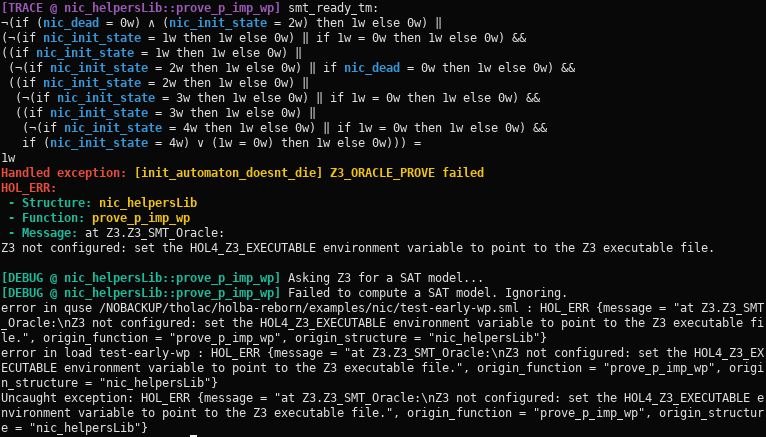
\includegraphics[width=\textwidth]{figures/loglib-ppexn-ppterm.png}
	\centering
	\caption{Extract of a script output, featuring \textit{trace} and \textit{debug} information from \textit{logLib} (Section \ref{loglib}), and an exception printed using the exception pretty-printer (Section \ref{pp_exn}). The original exception can be seen in white at the bottom of the image.}
	\label{loglib-ppexn-ppterm}
\end{figure}

\subsubsection{SML exception pretty-printer} \label{pp_exn}

As can be seen in Figure \ref{loglib-ppexn-ppterm}, default printing of HOL4 exceptions is not really easy to decipher. The is due to the fact that HOL4 has been designed as an \textbf{interactive} theorem prover to be used with \textit{Emacs}, which provides some layout and pretty-printing features. Therefore, a small pretty-printing library for SML exceptions has been implemented, called \textit{pretty\_exnLib}. It provides only two analogous functions that, given an exception as parameter, pretty-prints the exception and returns it unchanged. Listing \ref{pretty_exnLib_sig} presents the signature of the library, and Listing \ref{pretty_exnLib_usage} shows how it is used.


\subsection{Best practices for a complex platform} \label{best-practices-complex-platform}

When building complex systems, special care should be taken in order to ensure that it grows in good conditions. Despite providing the best capabilities, a system with poor usability will encounter a slow adoption, as shown in the previous section. But when a system gets used by an increasing number of users, a different working organization is needed. This section will first briefly introduce a critical concept that should be mastered for the successful growth of a software platform. Then, we will study the {CI} system that has been set up for HolBA.

\subsubsection{Developing simple interfaces}

In 1995, the Gang of Four published a book about design patterns for software design \cite{gamma_design_1995}. ``Program to an interface, not an implementation.'' is a key concept presented among the patterns. Since then, this sentence is considered as one of the most important design principles in software development.

This section doesn't intend to give a thorough explanation of the concept. However, some key insights shall be provided:

\begin{itemize}
    \item An interface is a contract between a system (such as a function, a library, a platform) and its user. This contract states the behavior and guarantees that this system offers via its public components. It defines the interaction between the component, the system, and the user. But most importantly, the contract leaves out the implementation. An interface builds an abstraction over the implementation. Using explicit contracts is particularly useful when performing contract-based verification, as it can simplify reasoning about components and allow building a more resilient system.
    \item Libraries provide features, which sometimes have a very complex implementation. This is particularly true for trustworthy binary code analysis. Building interfaces helps to abstract away complex implementations and helps to compose systems together.
    \item Programming to an interface instead of an implementation makes the code more resilient to changes. Indeed, if an implementation must be changed in order to provide more features, fix critical bugs or deliver more performance, codes that are not aware of the implementation will not need to be modified.
\end{itemize}

\subsubsection{Continuous Integration: tests and static analysis}

Continuous Integration ({CI}) is a development practice where developers of a project \textit{integrate} frequently their code and changes into a single shared source repository, hence the name of this practice. Each integration of any change into the shared repository should be automatically verified by automated builds and a full set of automated tests. This allows to immediately see if changes to the source repository break a feature or introduce a regression, thus allowing to fix it immediately. Since this practice imposes to run a whole battery of tests for each and every change, even the smallest one, automation is key. \cite{martin_fowler_continuous_nodate} gives a detailed introduction to this practice.

A CI system has been added to the HolBA repository, and its practices are being adopted by the research team. For each change, the CI system recompiles the whole platform from scratch and runs all the tests and executes a set of example scripts. Additionally, the CI system also performs some static analysis of the source code in order to give developers some key insight of the state of the code. Two static analyzers have been implemented, showing respectively the \textit{cheats} used in the formal proofs and the ``\textit{TODO}'' comments indicating left work to be done \footnote{At the time of writing, this feature has not been added yet to the CI system because of time constraints. However, it is ready to be integrated.}.

\section{Conclusions}

\subsection{Discussion}

The goal of this paper was to perform experiments about the automation of formal verification of devices at the binary level. The NIC model of \cite{haglund_formal_2016} has served as a central theme throughout the work. Work in this thesis has been divided in practice into three parts, in addition to the learning process due to the very steep learning curve of HOL4:

\begin{enumerate}
    \item \textbf{Implementation of the NIC BIR model}: the formal model of the NIC of \cite{haglund_formal_2016} has been partially implemented as a BIR program, and BSL has been added to the HolBA platform in order to make this task more convenient.
    \item \textbf{Non-proof-producing automatic contract verification library}: a user-friendly (adjective rarely used to describe HOL4), convenient and automatized library for contract verification have been implemented. This library brings HolBA one step closer to ``one-button solutions'' for performing software verification. It features a non-proof-producing translation of BIR expressions to expressions that can be exported to SMT solvers, and an extension of HOL4's SMT library has been realized in order to add reasoning about BIR memories.
    \item \textbf{Formal proof of a BIR program on a HOL4 state}: a novel usage of BIR and method for transferring properties from BIR program to formal HOL4 specification has been carried out. Additionally, while not automated, the work needed in order to implement automatic HOL4 tactics has been clearly identified. Every automation work should be preceded by a manual implementation of the task, that this proof intends to be.
\end{enumerate}

Throughout this work, a strong focus has been placed on ease of use and user-friendliness with BSL, the pretty-printer, the implementation of new logging utilities, guidelines about error handling in SML and with HOL4, and a friendly exception printer. We strongly believe that user experience of such complex platforms are of primary importance because it can dramatically reduce time spent in debugging and the need of exhaustive documentation. Furthermore, it can give users the desire to keep using the platform. If it is decided to put more work in HolBA in order to make it a powerful binary analysis platform, the research team is advised to consider this aspect while expanding HolBA capabilities.

Some failed experiments have also been realized, including the DepGraph tool that revealed to not be adapted to its planned usage or which would have needed to much work for too few benefits (though DepGraph's design is future-proof and the tool can easily be extended later if new needs or novel ideas appear), and the former two implementation attempts of the NIC model using flowcharts or C which have been found to not be suitable for device models.

\subsection{Future work}

The topic of software verification, while being as old as Computer Science, still have a lot of work to be done and paths to be explored. This thesis opens some paths that should be considered by someone interested in the topic.

The pretty-printer implemented in this work is only a small experiment only scratching the surface of what can be done in HOL4. Further work in this domain should follow the concrete needs that arise with extended usage of BIR. Current limitations and possible further work of the pretty-printer presented in this document include:

\begin{itemize}
    \item the generated output isn't parsable, which is against HOL4 conventions where every printed term should be parsable by HOL4 quoting system. A solution to this problem would be to implement a theory introducing definitions for the new abbreviations. However, some liberties taken in the pretty-printer cannot be parsed: (a) the flat printing of nested binary expressions of the same state, because they would need multiple arity functions which are not available in HOL4, and (b) \textbf{if-then-else} statements in the current representation.
    \item the pretty-printer doesn't use infix operators, feature widely employed in custom syntax used in some theories, like \textit{wordsTheory}. Infix syntax for binary operators can dramatically reduce the verbosity of expressions, and give a more familiar representation that \textit{could} be simpler to work with.
    \item the choice of colors could be reviewed in order to more closely follow HOL4 convention and usage. For example, BIR types are highlighted in the same color than free variables. While creating a very limited chance of ambiguities, users familiar with HOL4 conventions can be annoyed with this inconsistency.
\end{itemize}

The non-proof-producing contract verification library implemented in this work can be really useful for prototyping, but it cannot be used for trustful verification. The limitations it suffers could be reasonably fast to overcome, and they should be fixed especially if HolBA were to become a strong binary analysis platform. Limitations include (a) the impossibility to compose contract in order to reason about longer functions, to compose functions or to prove properties on not loop-free programs, and (b) the obvious limitation of not being proof-producing. Work is ongoing at the time of writing about weak-correctness and contract composition, answering to (a). The main blocker of (b) is the absence of a proof-producing ways of using SMT solvers for proving contracts (Equation \ref{eval_pre_imp_eval_wp}). The proof of Chapter \ref{trustful-nic-analysis} and its SML implementation identify what automatic procedures should be added to HolBA in order to perform step (b) and progress towards proof-producing automatic verification. Additionally, the signature of \texttt{prove\_contract} should be reworked in order to enable mixing it with proof-producing code, after both (a) and (b) are solved. For example, it should work with HOL4 definitions instead of raw terms.








































\end{multicols}

\renewcommand*{\bibfont}{\footnotesize}
\printbibliography

\newpage
\section*{Appendix. {\normalsize\textit{Figures}}}
\renewcommand{\thefigure}{A.\arabic{figure}}
\setcounter{figure}{0}

\begin{figure}[htbp]
	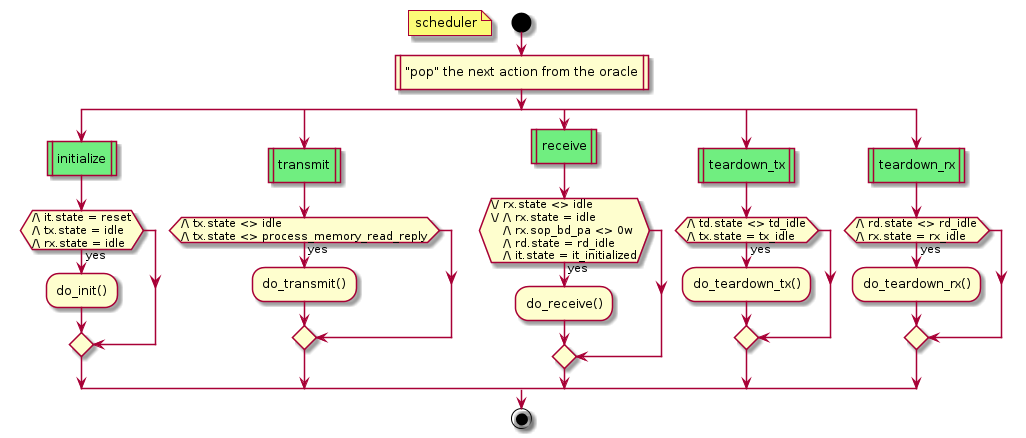
\includegraphics[width=\columnwidth]{figures/flowchart-scheduler.png}
	\centering
	\caption{Flowchart of the scheduler of the NIC model. Green nodes represent condition statements, here they represent the value of the popped action from the oracle. The full dot represents the entry point, and the other point the exit point.}
	\label{flowchart-scheduler}
\end{figure}

\begin{figure}[htbp]
	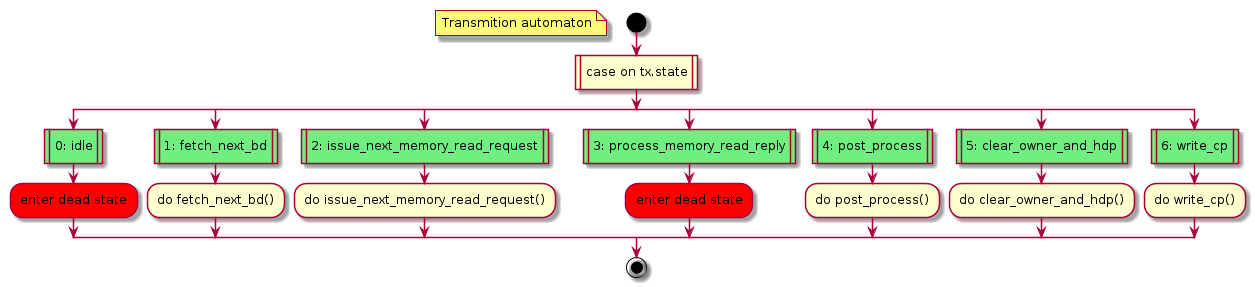
\includegraphics[width=\columnwidth]{figures/flowchart-tx.png}
	\centering
	\caption{Flowchart of the transmission automaton of the NIC model. Green nodes are similar to the ones of Figure \ref{flowchart-scheduler}. Red nodes represent non autonomous transitions leading to dead states.}
	\label{flowchart-tx}
\end{figure}

\begin{figure}[htbp]
	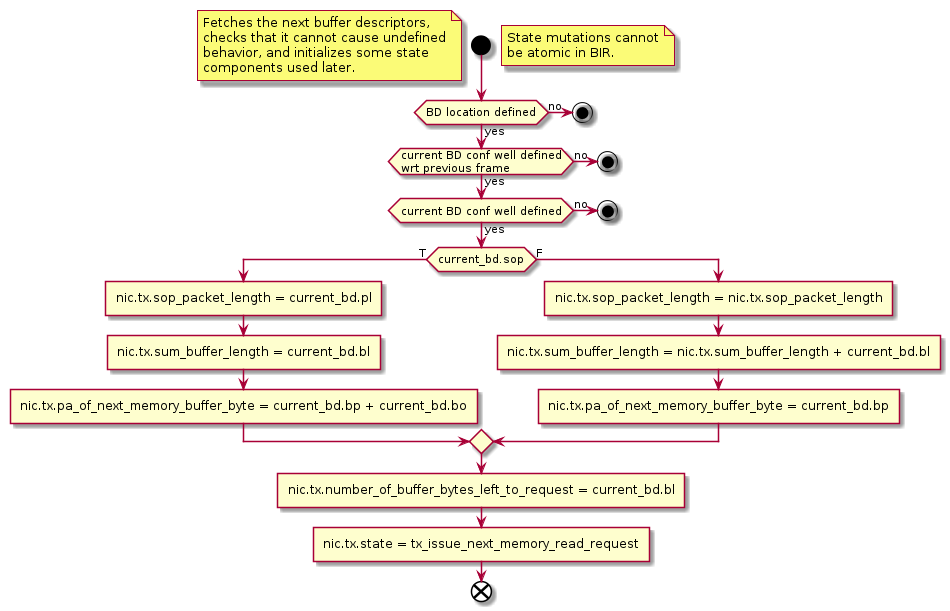
\includegraphics[width=\columnwidth]{figures/flowchart-tx_fetch_next_bd.png}
	\centering
	\caption{Flowchart of the \texttt{fetch\_next\_bd} transition of the transmission automaton of the NIC model. The full dot represent the entry point, $\bigotimes$ represents the exit point and the other dots are shorthands to represent dead transitions (the symbols have been changed because of technical limitations of the tool used to draw the diagram).}
	\label{flowchart-tx_fetch_next_bd}
\end{figure}

\end{document}























